\subsection{Extra}

% ================================================================================

\subsubsection{The Laplacian Pyramid \cite{laplacianpyramid}}
In order to compress an image reducing the pixel correlations the \textit{Laplacian Pyramid} was created: subtracting an image with its low-bass band filtered image (using a hand-crafted kernel) it's possible to reduce the variance and the entropy of the image itself; in this way less bits are necessary for representing the image.

The name is due to the similar result obtained applying a laplacian operator to an image.

The kernel used is a 5x5 gaussian-like kernel:
\begin{itemize}
    \item \textbf{separable}: $W(m,n) = \tilde{w}(m) \cdot \tilde{w}(n) $
    \item \textbf{symmetric}: $\tilde{w}(i)=w(-i), i \in [1,2]$, where $w(0)=a$, $w(1)=w(-1)=b$, $w(2)=w(-2)=c$
    \item \textbf{normalized}: $a+2c+2b=1$
    \item \textbf{equal contribution}: $a+2c=2b$
\end{itemize}
which leads to:
$$
W = \begin{cases}
    w(0)=a \\
    w(1)=w(-2)=\frac{1}{4} \\
    w(2)=w(-2)=\frac{1}{4} - \frac{a}{2} \\
\end{cases}
$$
Given $\alpha$ different kernel are created:
\begin{figure}[H]
    \centering
    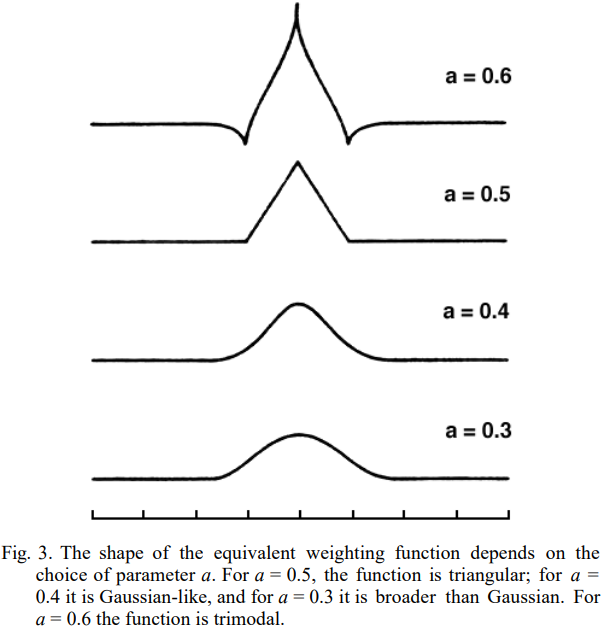
\includegraphics[scale=0.3]{laplacian-pyramid-kernels.png}
    \caption{Kernels as function of $\alpha$}
\end{figure}

Then, first, a \textbf{Gaussian pyramid} is created convolving the kernel with the image \textit{reducing} each time the spatial dimension then each low-bass band filtered image is subtracted with the low-pass band filtered image in the lower level (after \textit{expanding} it) creating a \textbf{Laplacian pyramid} where \textbf{high frequency information} are highlighted at different scales.

\begin{figure}[H]
    \centering
    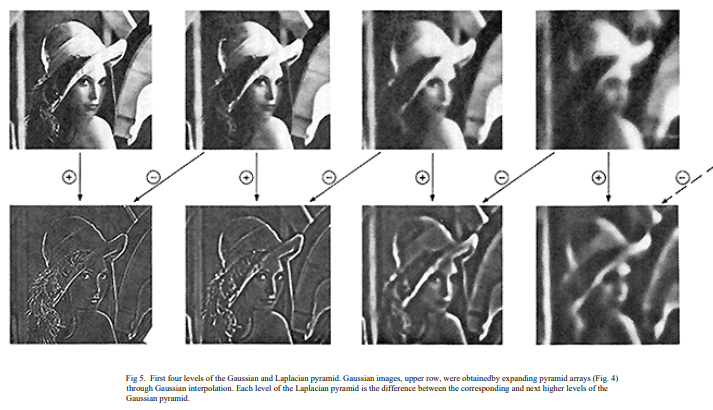
\includegraphics[width=\textwidth, keepaspectratio]{laplacian-pyramid-example.png}
    \caption{Laplacian pyramid example. The original image is the one on the left. Each image is REDUCED and EXPANDED for creating the Laplacian Pyramid.}
\end{figure}

The image can be reconstructed starting from the bottom level and expanding and summing two consecutive Laplacian images:
$$
g_l = L_l + EXPAND(g_{l+1})
$$

Further studies on the entropy and quantization allowed researcher to reduce much more the quantity  of information necessary for representing the image with a small loss in quality.

\begin{figure}[H]
    \begin{subfigure}{\textwidth}
        \centering
        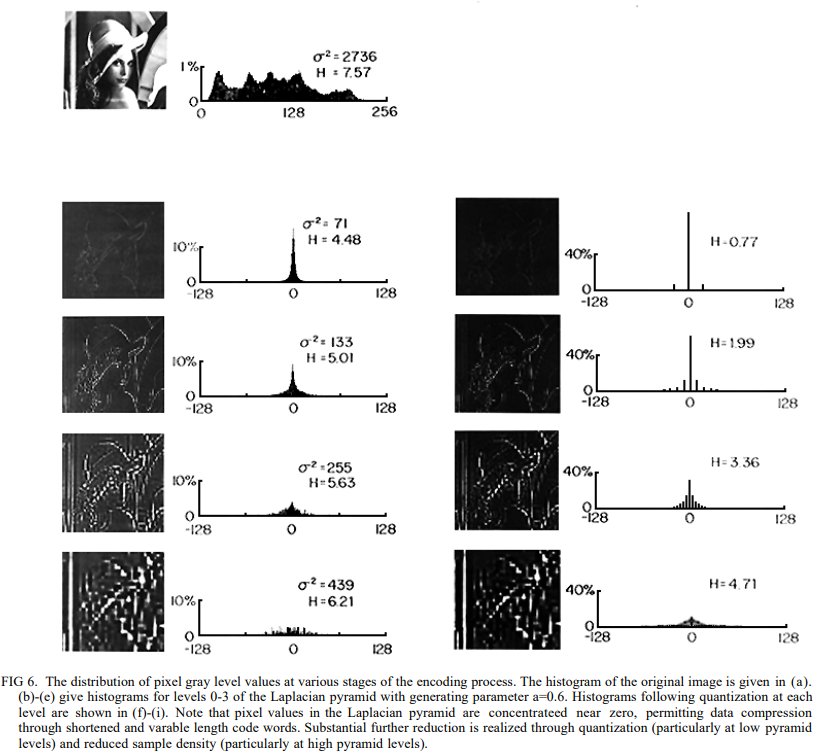
\includegraphics[scale=0.4]{laplacian-entrpy-quantization.png}
        \caption{Study on entropy and quantization on the Laplacian Pyramid.}    
    \end{subfigure}
    \begin{subfigure}{\textwidth}
        \centering
        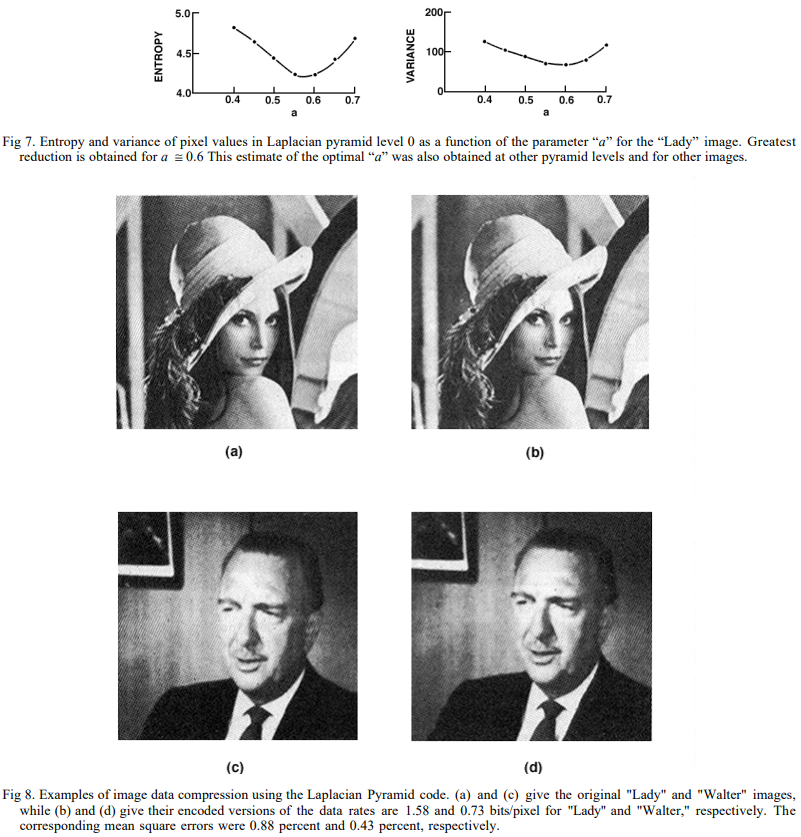
\includegraphics[scale=0.4]{laplacian-quantization-results.png}
        \caption{Examples with quantization using as width of bins a value such that there is a small degradation on the perception of the image at distance five times greater than the image dimensions.}            
    \end{subfigure}
\end{figure}
\newpage

% ================================================================================
\subsubsection{Identity mapping as output of the residual block \cite{resnetidentity}}
\begin{figure}[ht]
    \centering
    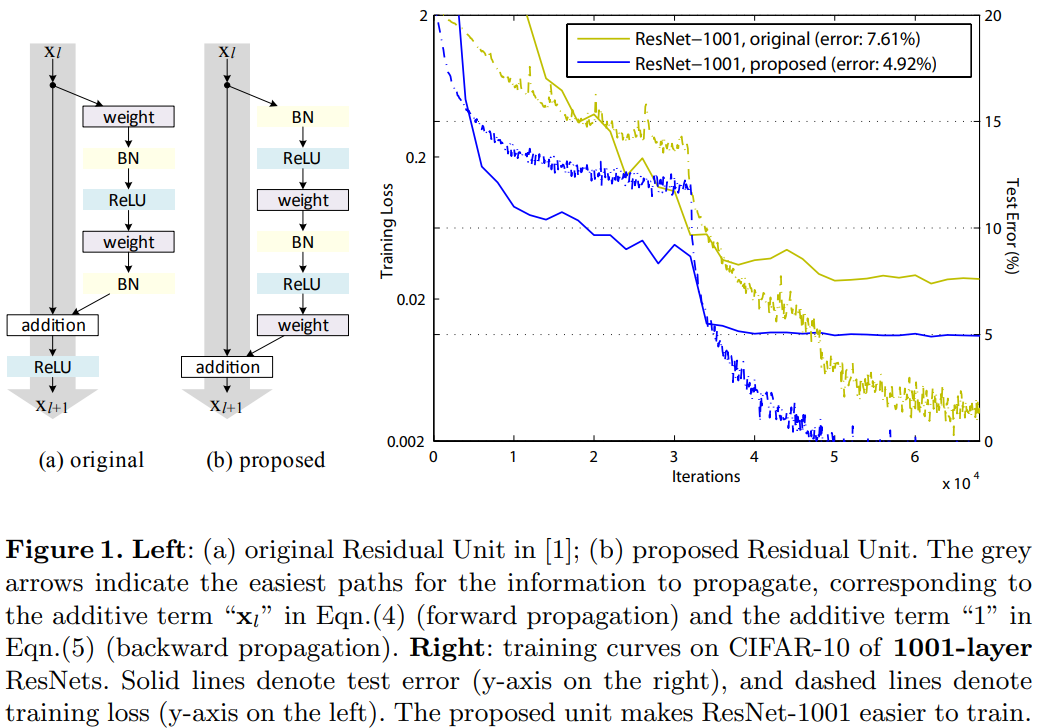
\includegraphics[width=\textwidth, keepaspectratio]{identity-results.png}
    \caption{The results of using a clean path in the identity.}\label{identity:results}
\end{figure}

The result [\Cref{identity:results}] shows that a \textbf{clean information path} from the input and the output (gray line in the figure) allows to ease the training improving the performance.

In order to to so an \textbf{identity mapping} should be used in the output of the residual block therefore the researcher proposed a new residual block where the input is \textbf{pre-activated}.

A \textit{Residual unit} can be formalized in this way:
$
\begin{cases}
    y_l = h(x_l) + F(x_l,W_l) \\
    x_{l+1} = f(y_l)
\end{cases}
$ where $x_l$ and $x_{l+1}$ are, respectively, the input and the output of the \textit{l-th} residual unit, $y_l$ is the output of the sum between \textit{h}, identity, and \textit{F} the residual, and f is the \textit{ReLU}.

Using an identity mapping in the output then $x_{l+1} = y_l = x_l + F(x_l,W_l)$ which recursively lead to $X_L = x_l + \sum_{i=1}^{L-1} F(x_i,w_i)$: any deeper unit $L$ is the sum of the input of a shallow unit $l$ and the residual of the unit between $l$ and $L$.

An intuition of why this is used in \Cref{lapsrn} and DRRN\cite{DRRN} can be seen in this results: since the skip connection allow to flow the real input (the LR image) than the network is able to take apart low frequency information better.

The backpropagation lead to:
$\frac{\partial\epsilon}{\partial x_l} = \frac{\partial\epsilon}{\partial x_L} \frac{\partial x_L}{\partial x_l} = \frac{\partial\epsilon}{\partial x_L} \left(1 + \frac{\partial}{\partial x_l} \sum_{i=l}^{L-1} F(x_i,W_i)\right)$
which is never 0 because is unlikely that $ \frac{\partial}{\partial x_l} \sum_{i=l}^{L-1} F(x_i,W_i)$ is always $-1$ for all minibatches.

\paragraph{Studies done on different residual block}
In order to prove the mathematical claims they experimented with different combination whose result are worse than the proposed residual block.

\begin{figure}[H]
    \begin{subfigure}{\textwidth}
        \centering
        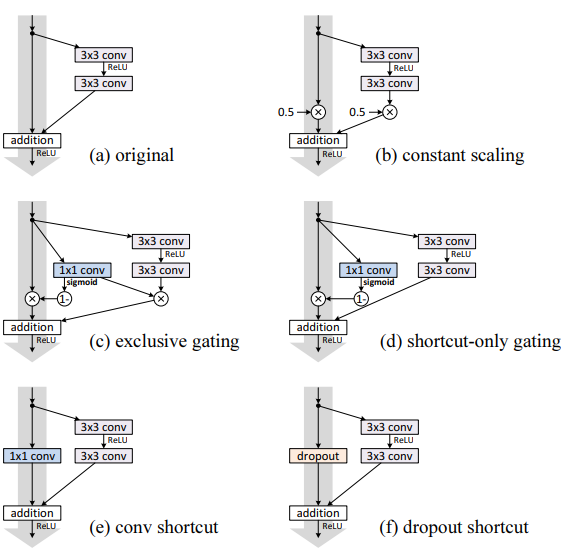
\includegraphics[width=0.5\textwidth, keepaspectratio]{Identity-wrong-identity.png}    
        \caption{The different combination tried.}
    \end{subfigure}
    \begin{subfigure}{\textwidth}
        \centering
        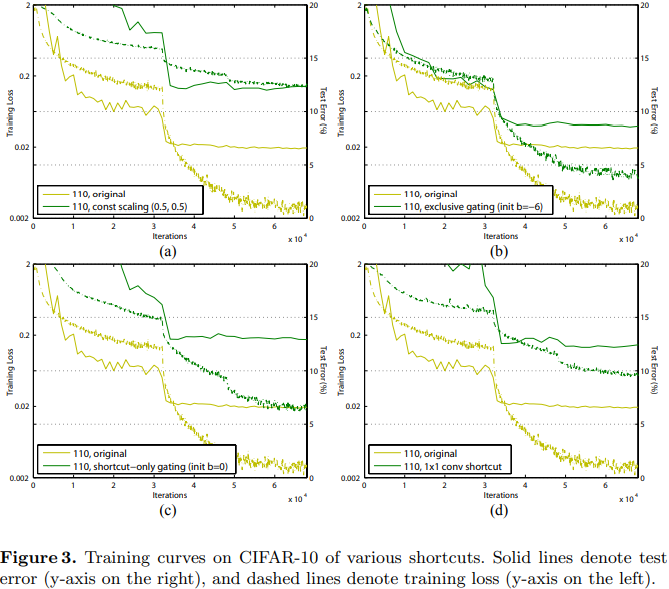
\includegraphics[width=0.5\textwidth, keepaspectratio]{Identity-what-they-tried-results.png}    
        \caption{The result of the different combination tried.}        
    \end{subfigure}
\end{figure}

\paragraph{Studies on the efffectiveness of the pre-activation}
The researchers experimentally prove the correctness of the pre-activation residual block.
\begin{figure}[H]
    \centering
    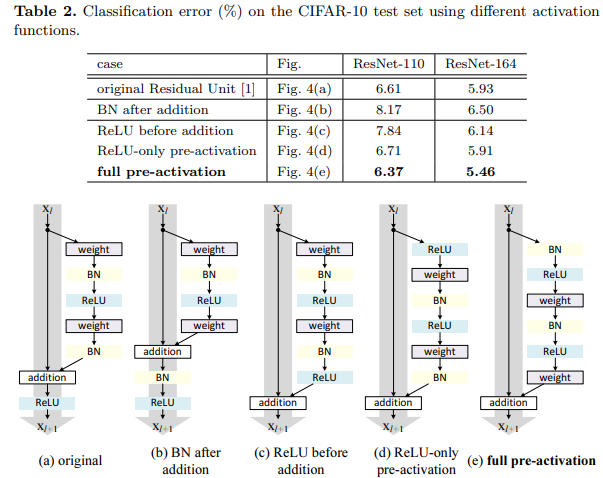
\includegraphics[width=\textwidth, keepaspectratio]{Identity-what-they-tried.png}
    \caption{Different combinations of disposition of batch normalization and ReLU}
\end{figure}

%====================================================================================

\subsubsection{Pixel Shuffle: sub-pixel convolution \cite{subpixelconvolution}}

The \textbf{Pixel Shuffle} rearrange the features $C \cdot r^2 \times H \times W$ learned into the LR space into $C \times r \cdot H \times r \cdot W$ activations learned into the HR space.

In \cite{eli5subpixelconvolution}, the authors proved that transposed convolution and subpixel convolution return the same result and convolving the features map with a convolution ($r^2 \cdot C_{out}$, $C_{in}$, $k_H$, $k_W$) where r is the upscale factor and then rearrange the activations in order to have an activation whose size is $(r \cdot H, r \cdot W)$ is the same as apply a transposed convolution ($C_{out}$, $C_{in}$, $r \cdot k_H$, $r \cdot k_W$)  ( fractional strided convolution where the input is modified inserting zeros in between and padded in order to have an output upscaled with respect the input) 